%!TeX root=../../master.tex
\section{Detecting Points}\label{sec:detecting-points}

We have desgined the system in wuch a way, that the user must point at the smart device he desires to control before he performs a gesture.

Pointing at a smart device informs the system which device actions should be sent to. This allows multiple devices to share actions and only the device being pointed at, will be receive the action. Configuring multiple devices with the same gesture means that the users can configure fewer gestures as they can be reused.

We define a point as the user holding his phone still for a small period of time. 
An accelerometer can be used to detect if the user holds the device still. 
If there is a low amount of activity on all three axes, 
it is assumed that the user is holding the device in his hand without moving it.

\Cref{fig:point-to-gesture-state-diagram} shows the relationship of a point and a gesture in a state diagram. 
All gestures begin and end with a point. 
When the first point is detected, 
we intrduce a very short delay in order for the user to prepare to do the gesture, 
\eg move the position of his hand. 
The delay was added because from our testing we found that if there was no delay, the recognition would suddenly begin without the user being prepared, resulting in the first data being invalid and not part of any gesture and ultimately the gesture would not be recognized.
The gesture recognition begins when the delay has passed. 
Gestures are recognized using the previously described \$3 Gesture Recognizer. 
After the gesture has been performed, 
the device must be held still again and the second point is detected. 
The collected gesture data is then analyzed by the \$3 Gesture Recognizer, 
in order to determine which known gesture was performed, if any at all. 
Lastly, the system returns to the initial state and another gesture can be performed.

While performing the gesture, the recognition may timeout. 
The \$3 Gesture Recognizer can recognize gestures for a maximum of four seconds before the recognition is canceled. 
In such case, the system returns to the initial state.

\begin{figure}[h]
\centering
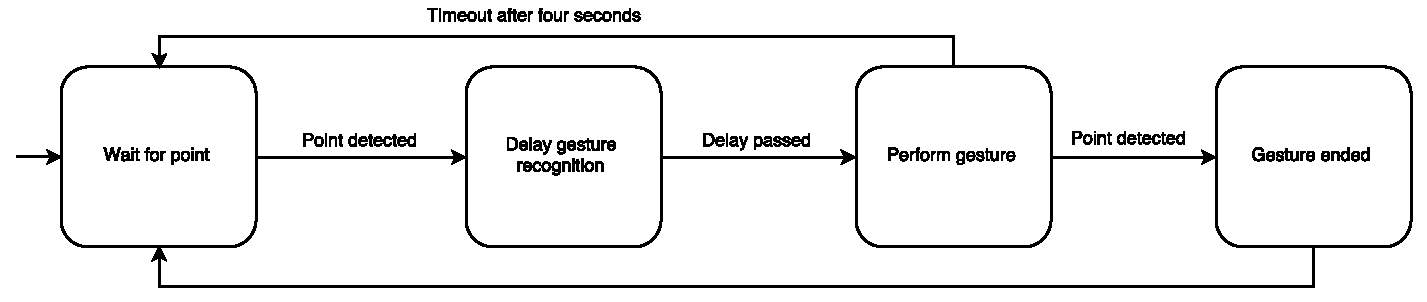
\includegraphics[width=\textwidth]{images/point-to-gesture-state-diagram}
\caption{State diagram showing the relationship between a point and a gesture. A gesture always starts and ends with a point.}
\label{fig:point-to-gesture-state-diagram}
\end{figure}

\subsubsection{Using Accelerometer Data to Detect a Point}

\Cref{fig:pointer} shows screenshots of an application, 
that we created to experiment with data from the accelerometer. 
The figure shows graphs of measurements made while the device was lying on a table (\Cref{fig:pointer:table}), 
the user, a young male, was pointing with the device in his hand (\Cref{fig:pointer:hand}), 
and while the user was walking with the device in his hand (\Cref{fig:pointer:walk}).
We measure this so that we do not recognize a device laying still on a table, 
as a user pointing.
 
The $x$-, $y$- and $z$-values are measured in radians per second. 
The $y$-axis of the graph spans from \num{-5} to num{5}. 
The graphs shows that there are small, 
but measurable differences between the measurements made when the device is lying on the table,
and when the user is pointing with the device. 
This allows us to distinguish between the two scenarios, 
and disregard measurements made when the device is lying on the table. 

Furthermore the graphs clearly shows that there is a measurable difference between the values read when a user is pointing with a device, 
and walking with the device in his hand. 
Based on this small experiment, 
we can conclude that the accelerometer data can be used to determine if a user is pointing with a device.

\begin{figure}[!htb]%
    \centering
    \subbottom[Table]{\label{fig:pointer:table}
        \frame{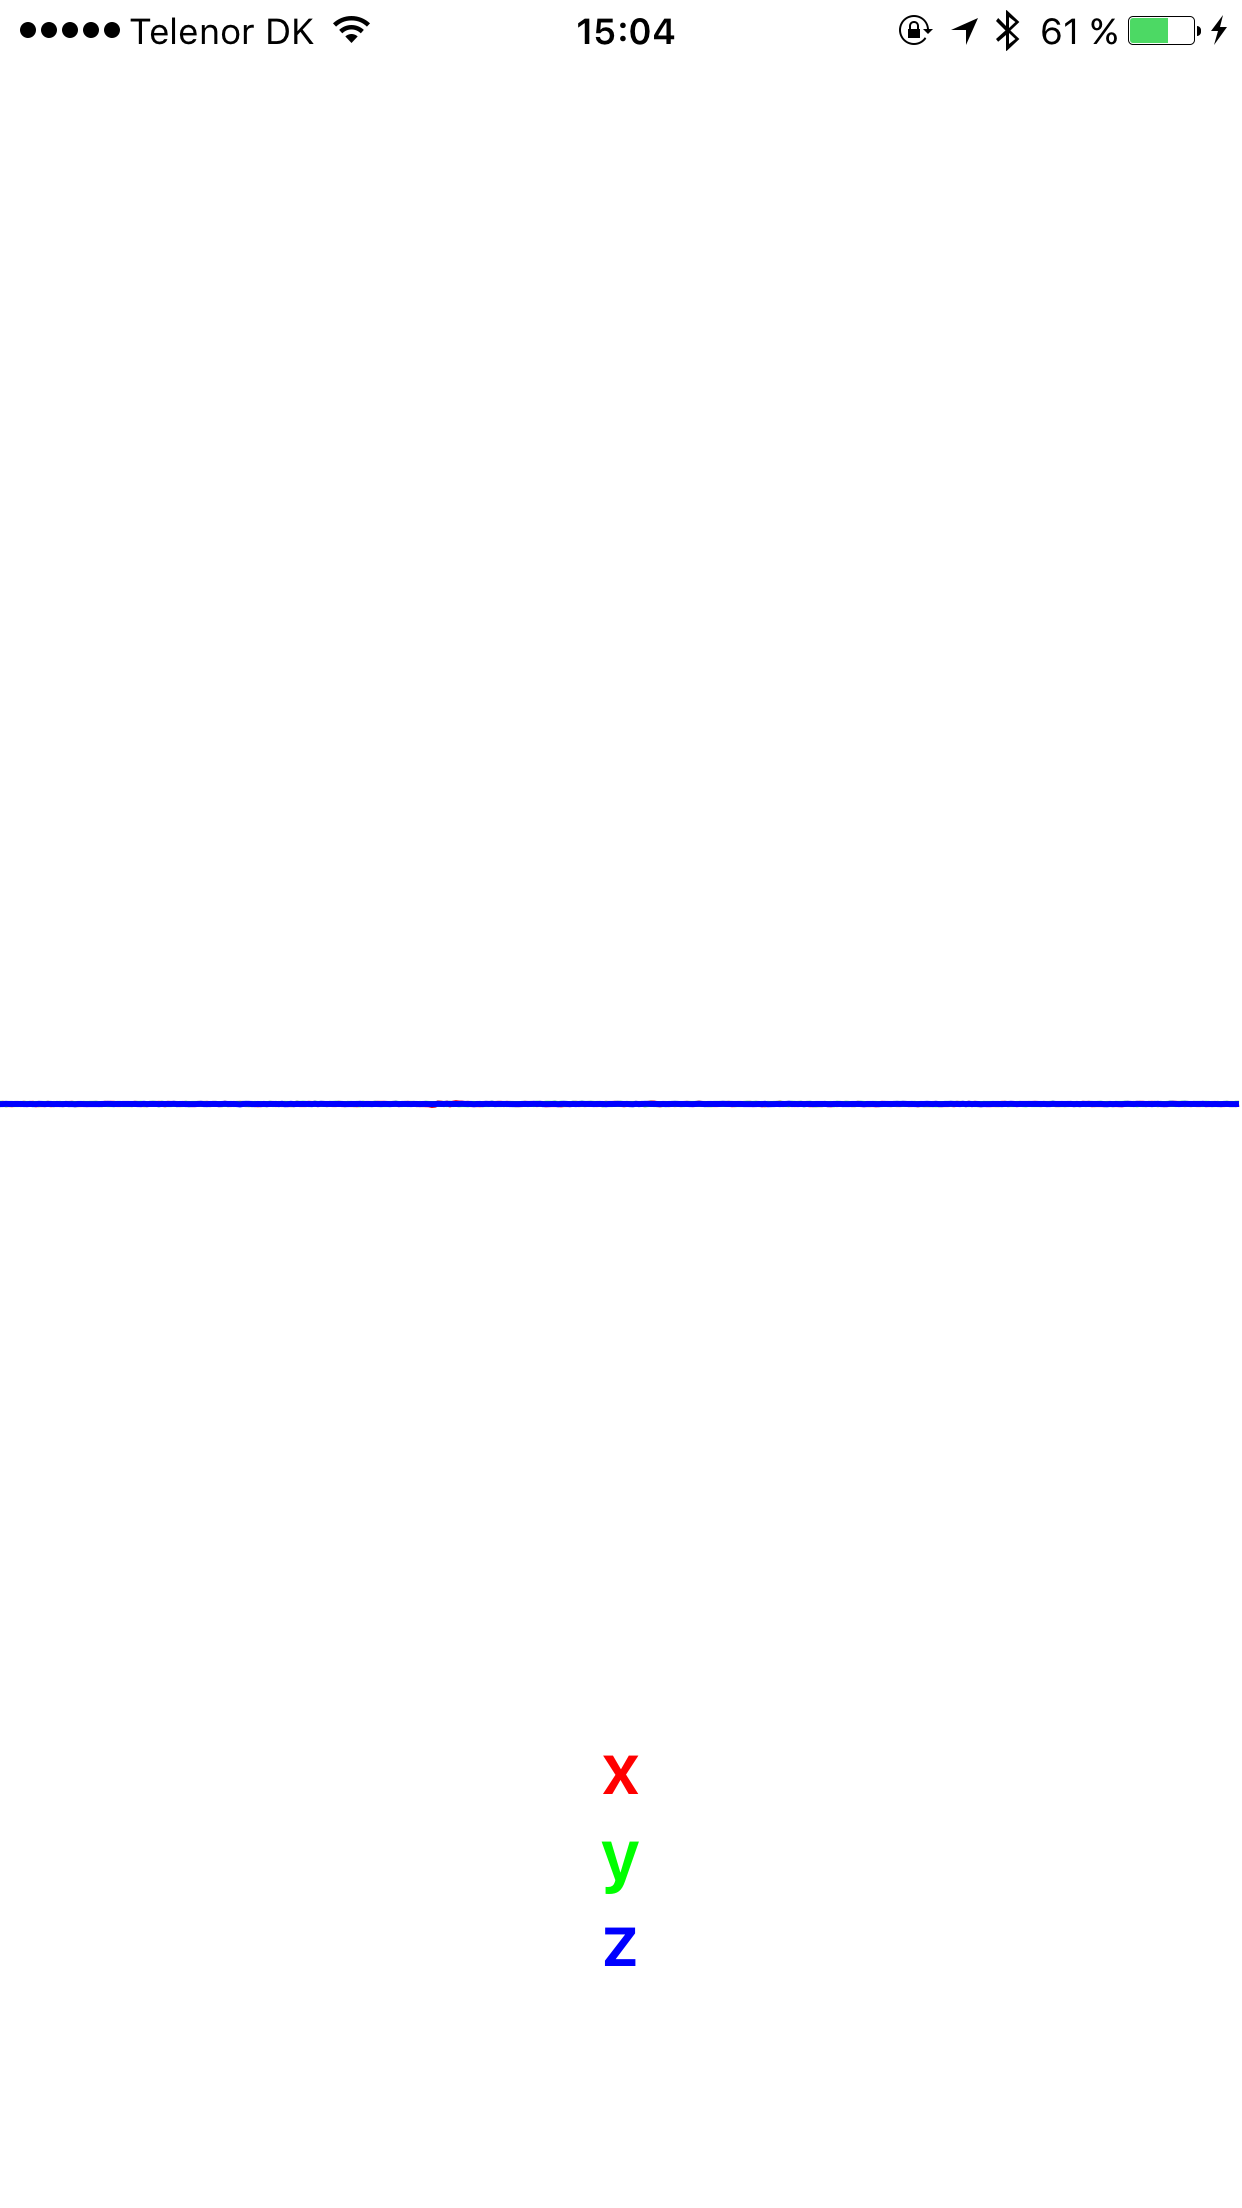
\includegraphics[width=0.3\textwidth]{images/pointer-table}}
    }
    \subbottom[Hand]{\label{fig:pointer:hand}
        \frame{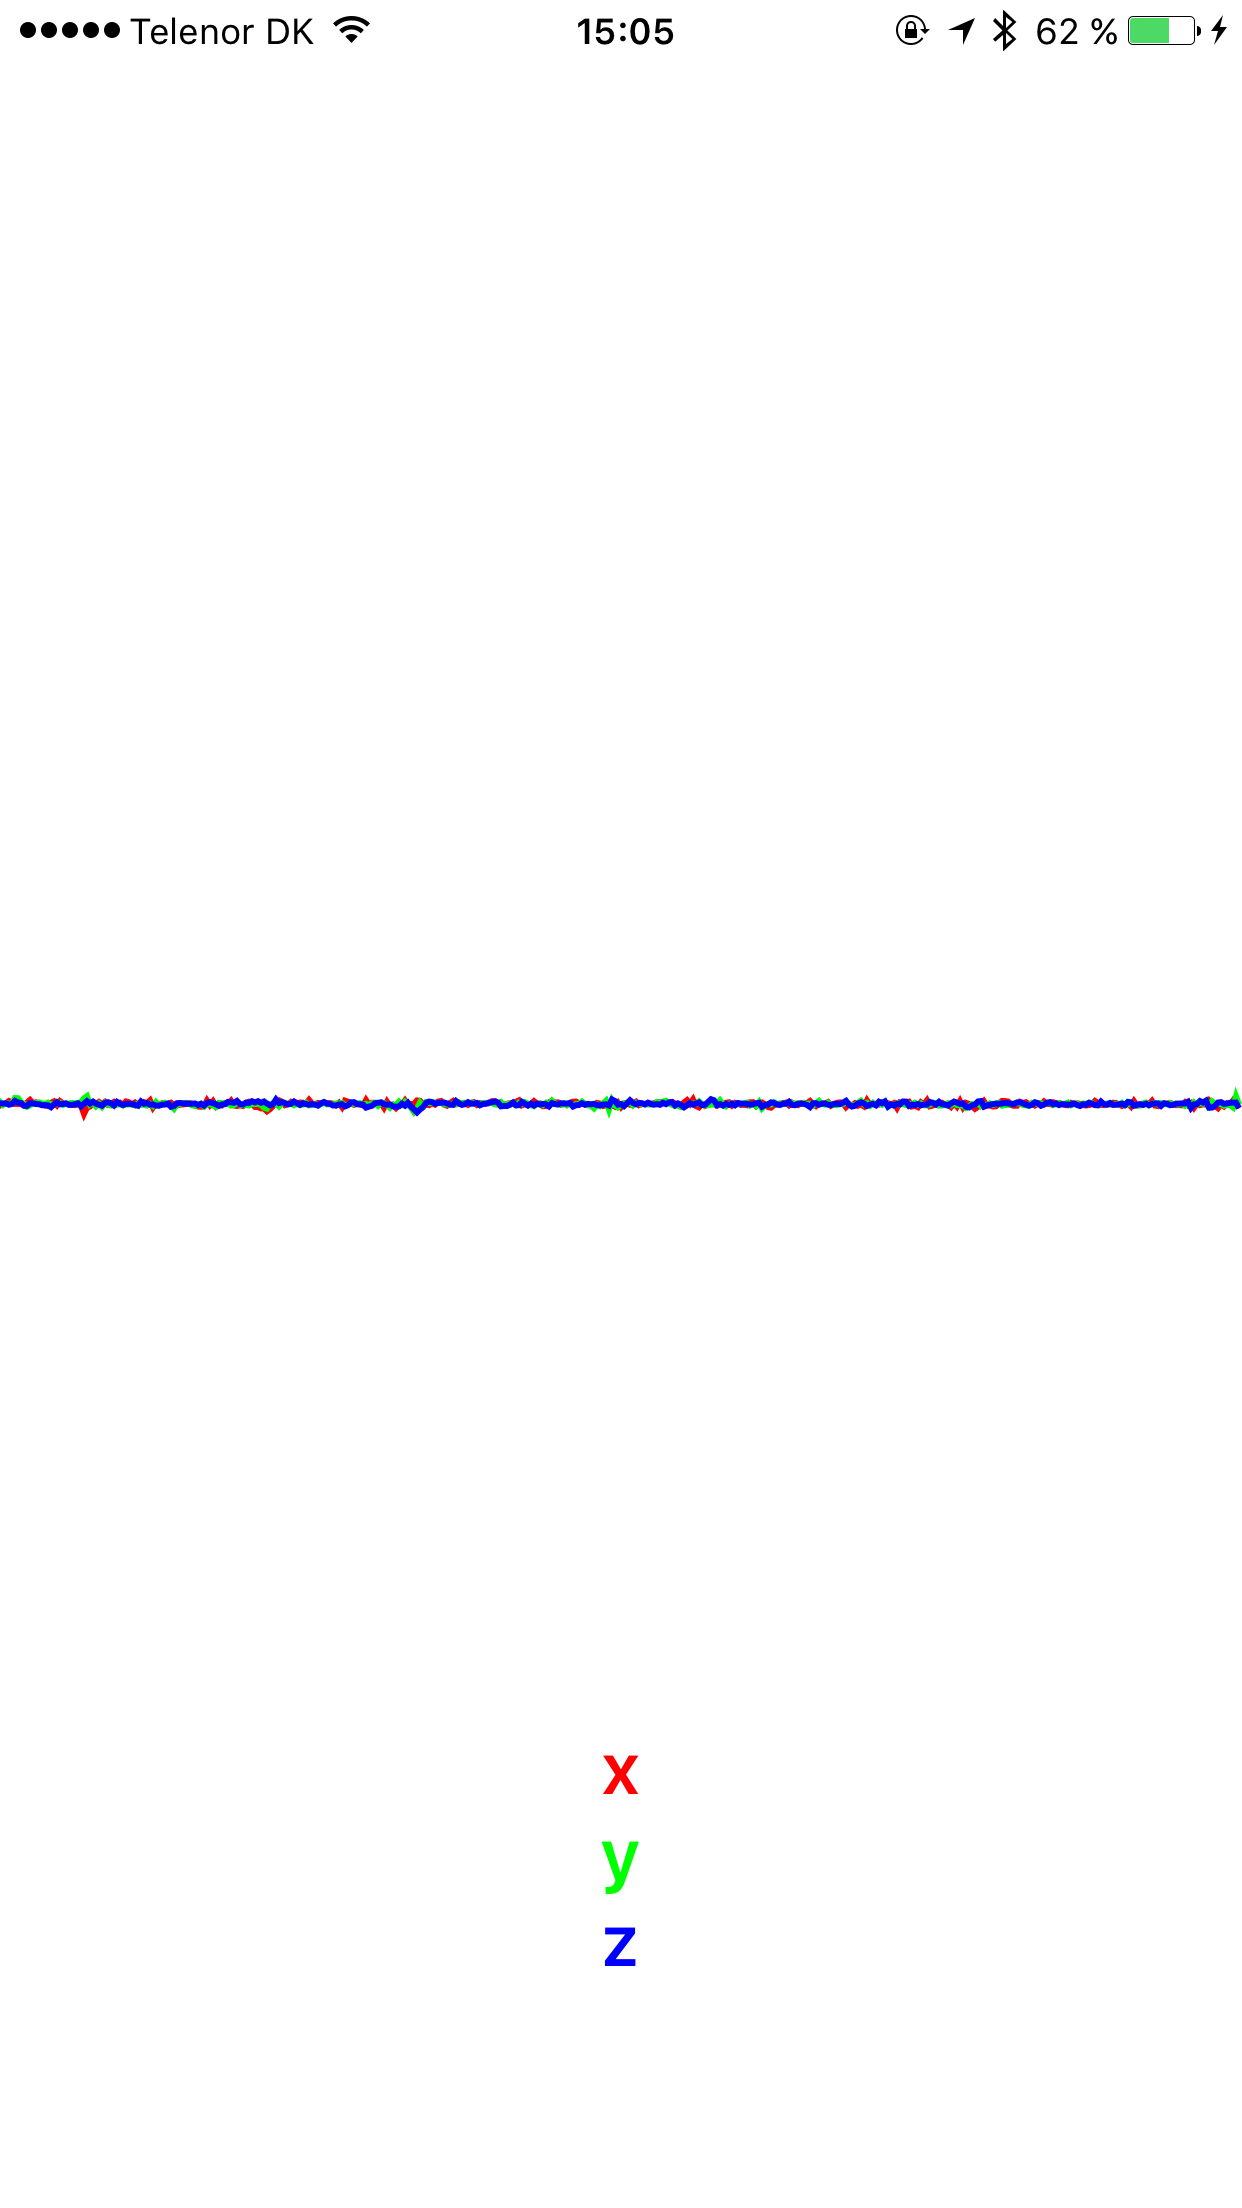
\includegraphics[width=0.3\textwidth]{images/pointer-hand}}
    }
    \subbottom[Walk]{\label{fig:pointer:walk}
        \frame{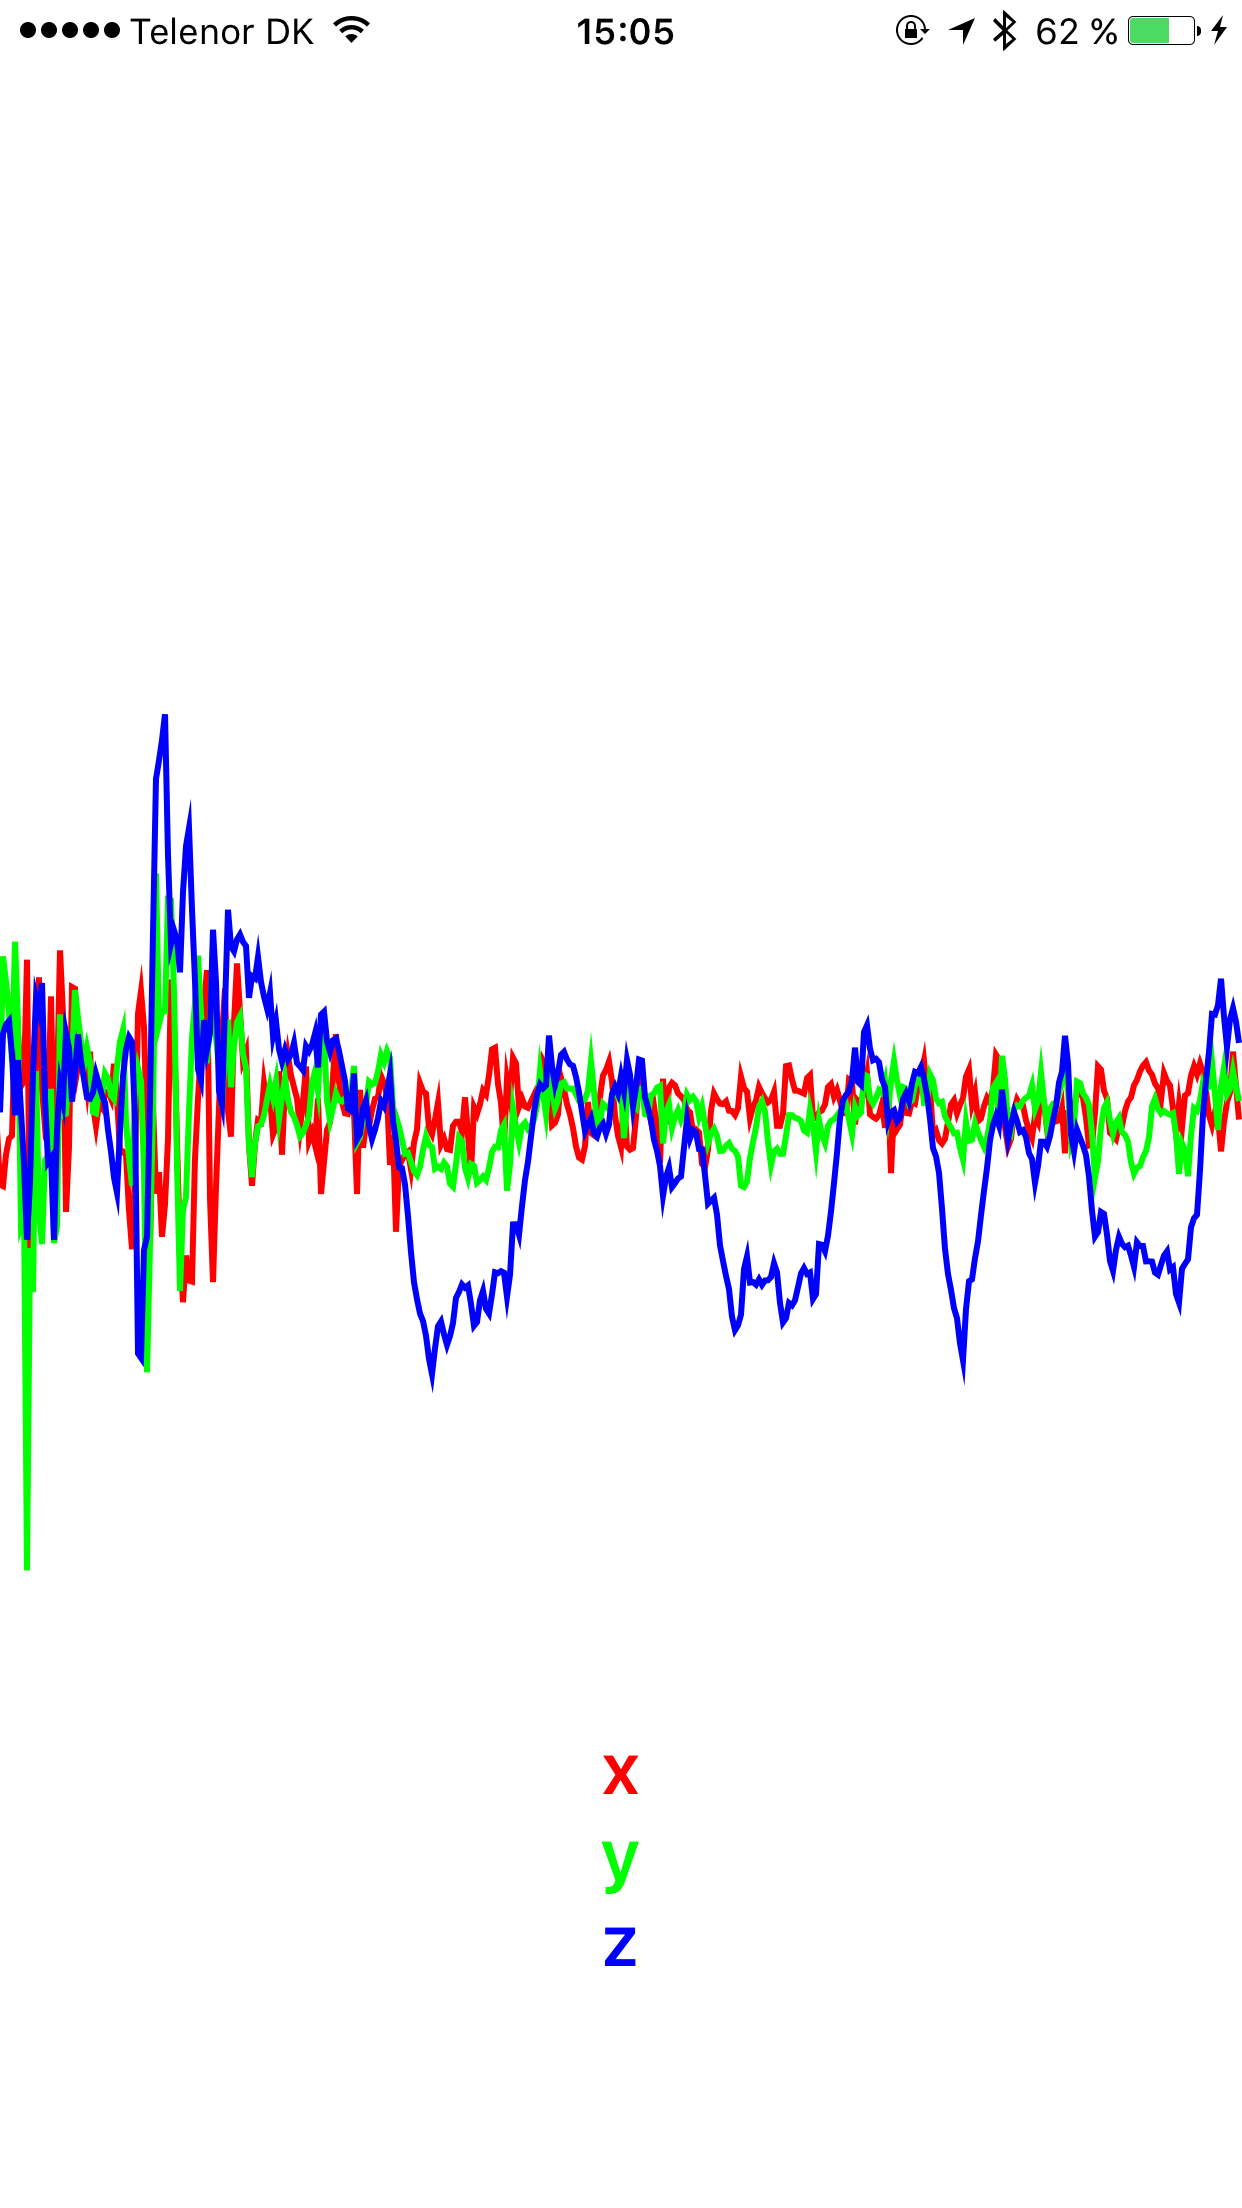
\includegraphics[width=0.3\textwidth]{images/pointer-walk}}
    }
    \caption{Screenshots of application created to experiment with data from the accelerometer. Leftmost screenshot shows graph of measurements made when the device lies on a table. The middle image shows graph of measurements made while pointing with the device. Rightmost screenshot shows graph of measurements made while the user was walking with the device in his hand.}
    \label{fig:pointer}
\end{figure}

\subsubsection{Detecting Points using PointDetector}

Part of the gesture recognition involves detecting if a user points. 
In order to limit the scope for the initial prototypes of the solution, 
we limit the context in which a point is detected, 
to a user walking with the phone in his hand, 
then stopping up to point at an actuator with the phone.

We created the \texttt{PointDetector} class and instances of this receives data from the accelerometer, 
and based on the data it determines if a user points with the device. 
When a user points with the device, 
an instance of the class will inform a listener, i.e. another object interested in knowhing if the user points.
Data from the accelerometer is expressed as acceleration on the $x$, $y$ and $z$ axes.

The state diagram in \Cref{fig:pointdetector-state-diagram} illustrates the internals of the \texttt{PointDetector} class. 
When instantiated, the object will not be detecting, 
\ie it will not be receiving accelerometer data. 
After the instantiation, the instance can begin detecting. 
The detection can be stopped at any time.

When detecting, the \texttt{PointDetector} will wait for the first acceleration data from the accelerometer, 
that indicates that the user is pointing. 
When the it is received, 
the object will enter the \textit{Sampling} state, 
in which it continuously checks data from the accelerometer, 
to determine if it indicates a point. 
If it indicates a point, 
both the \emph{point sample count} and the \emph{total sample count} will be incremented. 
If the data does not indicate a point, 
only the total sample count will be incremented.
%Thalley: Beskrivelse af de her sample counts bør nok ligge heroppe. Kunne ikke lige finde en pæn måde at gøre det på selv.

At the same time the detector enters the sampling state, 
it will start a timer that runs for a number of seconds. 
When the time has passed, 
the detector will leave the sampling state, 
and determine if the result of the sampling, 
indicates that the user is pointing. 

The sampling phase is necessary in order to avoid ``outliers'', 
\ie anomalies in the accelerometer data. 
The accelerometer continuously delivers data, 
and the acceleration may indicate that the user is pointing. 
However, it may not be the users intention to point at all. 
It may be that he just held the device very still for a short moment.

In order to determine if the result of the sampling phase indicates a point, 
the detector investigates the relation between the point sample count, $p$, 
and the total sample count, $t$. 
If $p/t \geq c$, where $c$ is the necessary percentage of samples that must indicate a point, 
then the detector can conclude that the sample is indeed a point.

After the sampling phase has concluded, 
the detector will wait for the next data from the accelerometer that indicates a point.

An accelerometer delivers an $x$-, $y$- and $z$-acceleration. 
Determining if acceleration data indicates a point is a matter of checking if the three values fits within some threshold, $h$. 
In order to check if the phone is lying still on a table, 
the values must be checked against another threshold, $g$. Note that $g < h$.

\begin{figure}
\centering
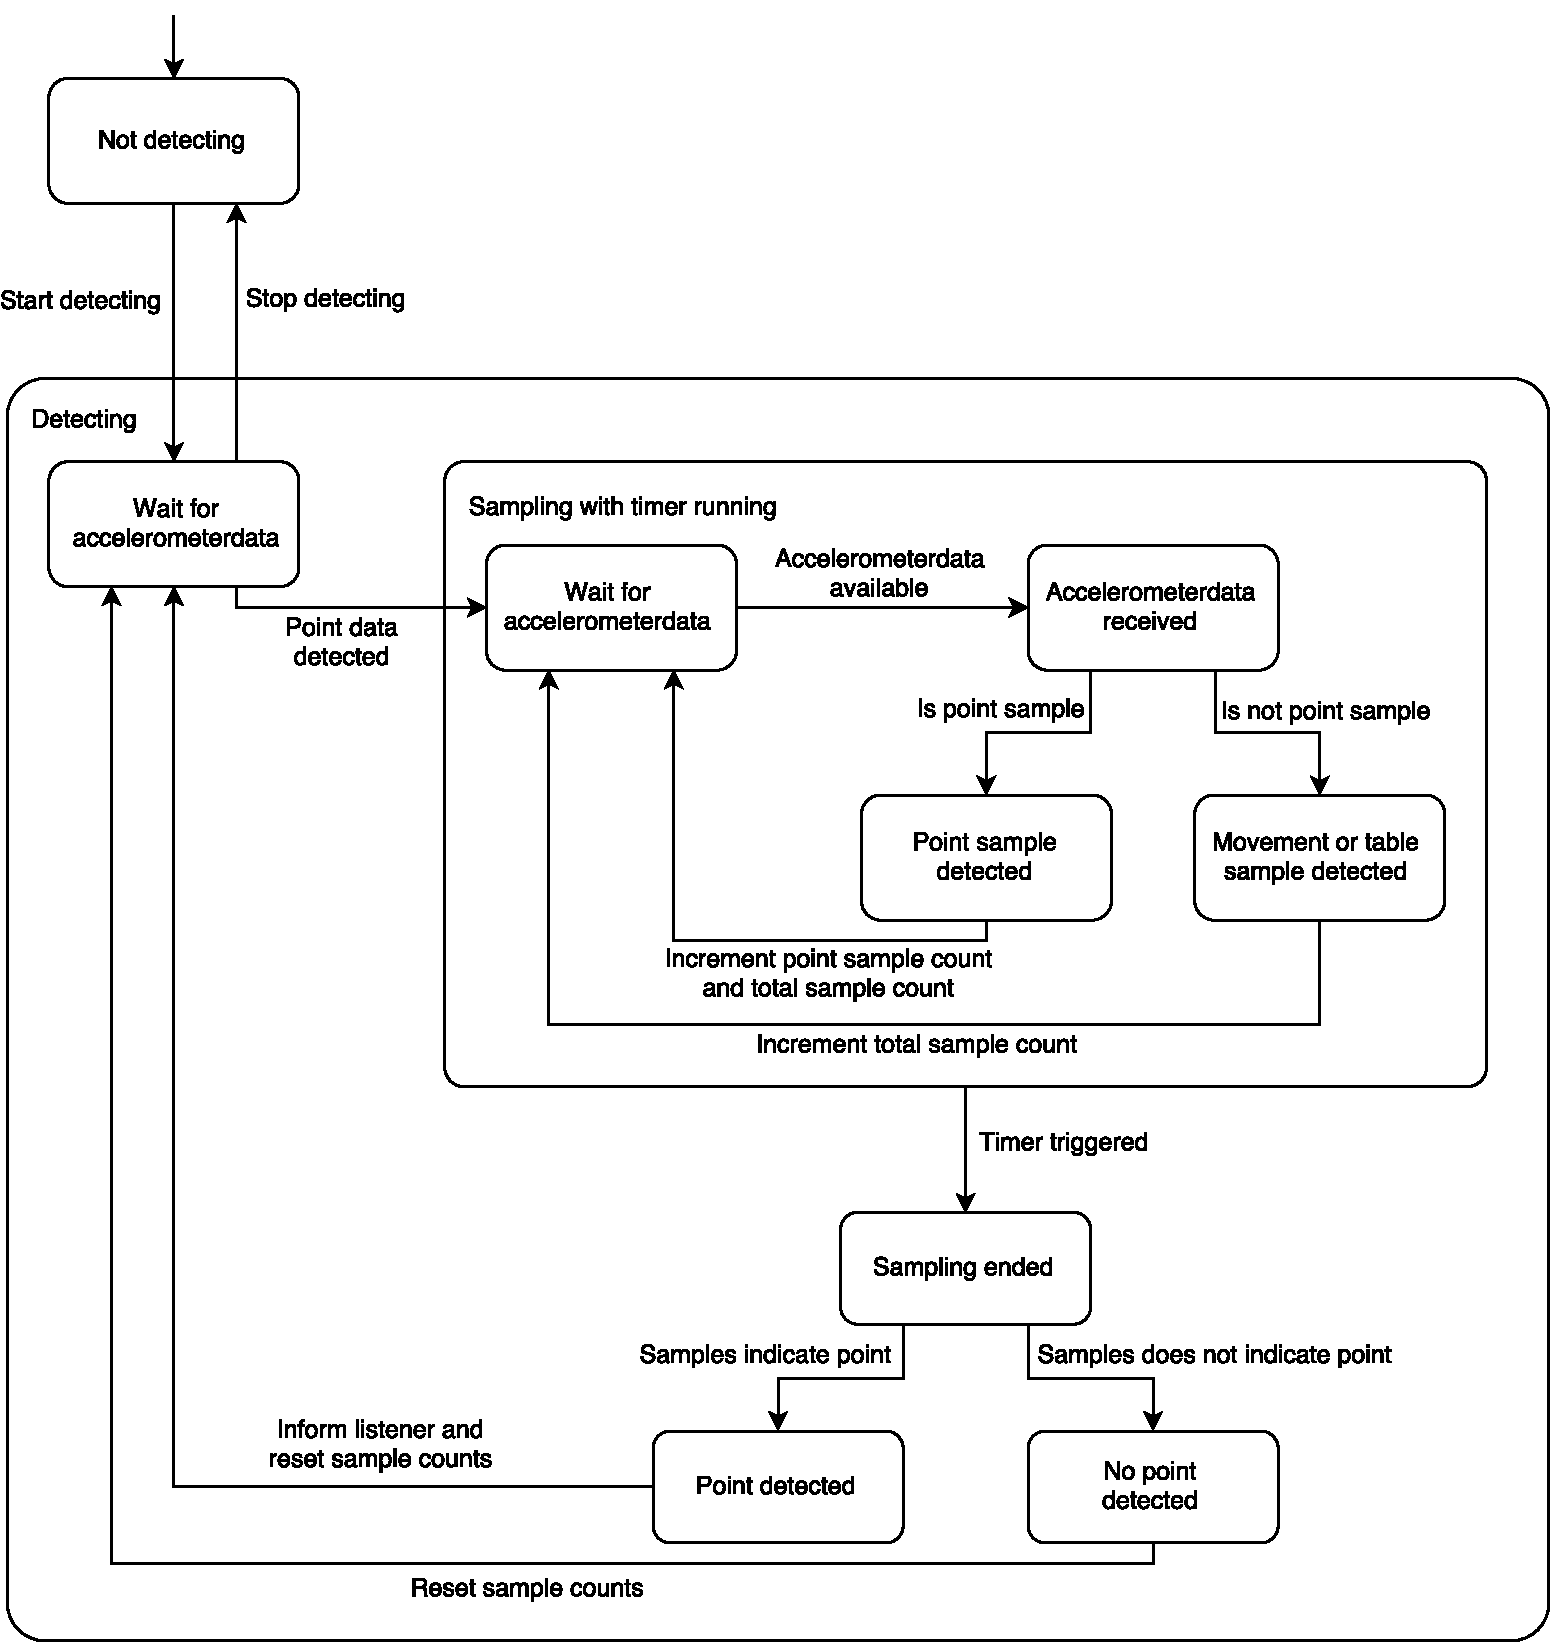
\includegraphics[width=\textwidth]{images/point-detector-state-diagram}
\caption{State diagram showing the states the \texttt{PointDetector} class can be in.}
\label{fig:pointdetector-state-diagram}
\end{figure}

The following pseudo code checks if acceleration data from the accelerometer indicates a point. 
\texttt{DataFitsWithinThreshold} takes the data from the accelerometer and a threshold $t$. \\
The function returns whether or not all of the $x$-, $y$- and $z$-values in the accelerometer data fits within the threshold.

\begin{algorithm}
  \begin{algorithmic}
    \Function{DataFitsWithinThreshold}{$data$, $t$}
      \State \Return $data.x \leq t \And data.x \geq -t \And data.y \leq t \And data.y \geq -t \And data.z \leq t \And data.z \geq -t$
    \EndFunction
  \end{algorithmic}
\end{algorithm}

The function \texttt{AccelerometerDataIndicatesPoint} takes data from the accelerometer data, 
and checks if it fits within the threshold $g$, 
indicating that the data comes from a device lying on the table. 
If the data fits within $g$, 
the function returns false. 
If it does not fit within the threshold $g$, the function checks if the data fits within the threshold $h$ and returns the result of the check as a boolean value. $h$ is some small number that represents an approximate of the acceleration of the device when the user points with it.

\begin{algorithm}
  \begin{algorithmic}
    \Function{AccelerometerDataIndicatesPoint}{$data$}
    \If{\Call{DataFitsWithinThreshold}{data, g}}
    \State \Return \texttt{false}
    \Else
    \State \Return \Call{DataFitsWithinThreshold}{data, h}
    \EndIf
    \EndFunction
  \end{algorithmic}
\end{algorithm}

\Cref{fig:pointdetector-uml} shows an example of the attributes and operations the \texttt{PointDetector} may have. 
Most of the attributes and operations should be self-explanatory but some may need a short description.

\begin{itemize}
  \item \texttt{pointingDuration} specifies the duration of the timer registered when entering the sampling phase.
  \item \texttt{pointingSampleFrequency} corresponds to $c$, the percentage of samples that must indicate a point.
  \item \texttt{pointingThreshold} corresponds to $h$, the threshold of data when determining if the device is lying on the table.
  \item \texttt{tableThreshold} corresponds to $g$, the threshold of data when determining if the device is being pointed with.
  \item \texttt{pointDetectedCallback} is a closure called when a point is detected.
\end{itemize}

By trial and error we found the following thresholds to be suitable:

\begin{itemize}
\item \texttt{pointingDuration} = 0.5
\item \texttt{pointingSampleFrequency} = 0.5
\item \texttt{pointingThreshold} = 0.05
\item \texttt{tableThreshold} = 0.005
\end{itemize}

The thresholds were determined by adjusting the values, 
until an acceptable behavior was achieved. 
No systematic experimentation of the values were performed, 
as we have a hypothesis that the values can be calibrated for each user. 
For example, we found that \texttt{pointingThreshold} to be dependent of the user. 
It depends on how much the user shakes, 
when trying to hold his hand still. 
A solution is to use a value higher than the values measured when he is holding his hand still.
However, the lower the threshold is, 
the better we can detect a point.

\begin{figure}
  \centering
  \begin{tikzpicture} 
    \umlclass[x=0,y=0]{PointDetector}{
    +/- isDetecting: Bool\\
    - isSampling: Bool\\
    - pointingDuration: Float\\
    - pointingSampleFrequency: Float\\
    - pointingThreshold: Float\\
    - tableThreshold: Float\\
    - samplingTimer: Timer\\
    - pointingSampleCount: Int\\
    - totalSampleCount: Int\\
    - pointDetectedCallback: Closure
    }{
    + beginDetecting()\\
    + endDetecting()\\
    - didReceiveAccelerometerData(data: AccelerometerData)\\
    - accelerometerDataIndicatesPoint(data: AccelerometerData): Bool\\
    - dataFitsWithinThreshold(data: AccelerometerData, threshold: Double): Bool\\
    - samplingTimerTriggered()
    } 
  \end{tikzpicture}
  \caption{Class diagram of the \texttt{PointDetector} class.}
  \label{fig:pointdetector-uml}
\end{figure}

%%% Local Variables:
%%% mode: latex
%%% TeX-master: "../../master"
%%% TeX-command-extra-options: "-shell-escape"
%%% End:
